\section{实验结果及分析}

\subsection{仿真结果}

使用发布包提供的矩阵乘法测试程序（shell1/matrix\_mult.c）进行行为仿真，通过Trace比对机制验证Cache实现的正确性。测试程序覆盖了大量的lw/sw/lb/sb/lh/sh指令，能够充分检验i\_cache和d\_cache的读写逻辑。

仿真完成后，TCL控制台输出如下图所示：

\begin{figure}[htp]
    \centering
    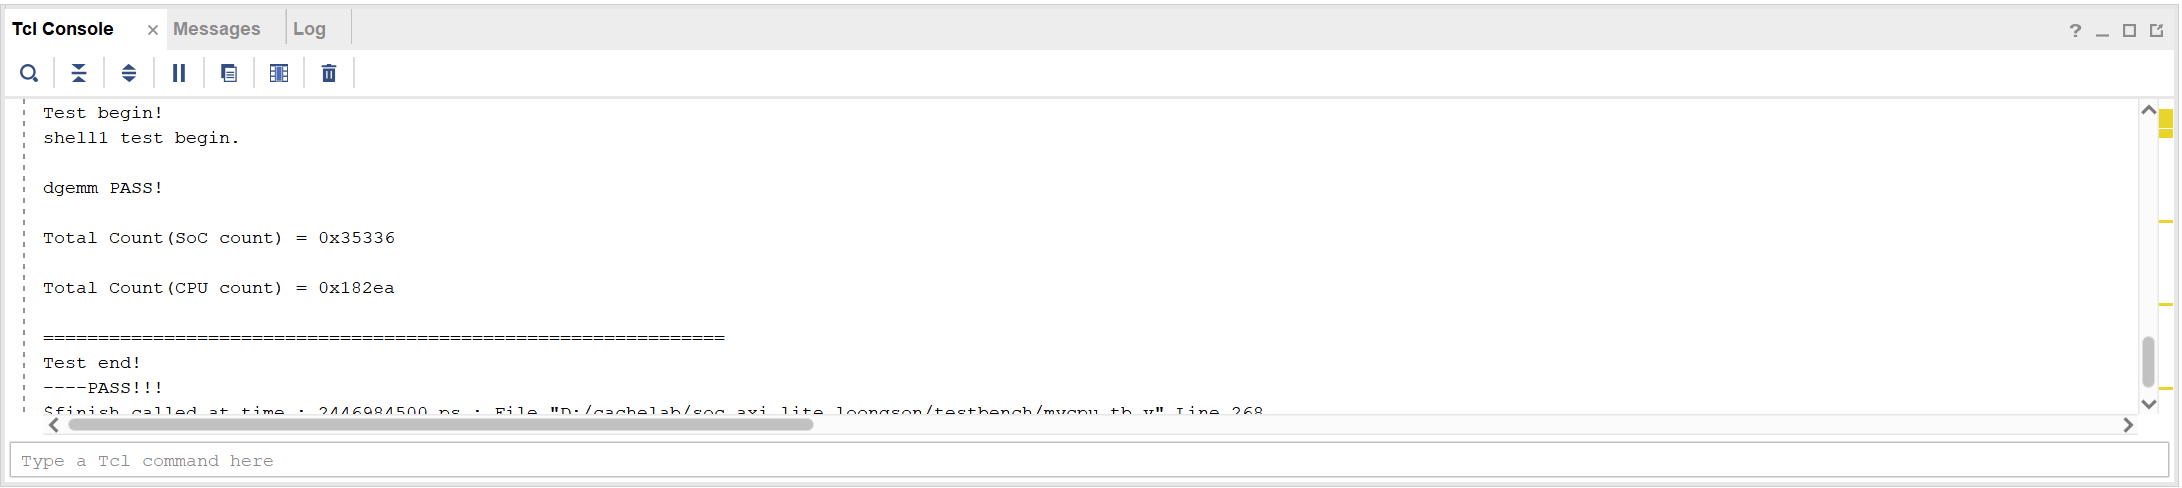
\includegraphics[width=0.95\textwidth]{image/tcl_console.png}
    \caption{仿真TCL控制台输出：\texttt{----PASS!!!}（仿真时间2446984500 ps，err\_count=0）}
    \label{fig:console}
\end{figure}

控制台关键输出：
\begin{itemize}
    \item \texttt{Test begin!}：testbench启动；
    \item \texttt{shell1 test begin.}：矩阵乘法测试程序开始执行；
    \item \texttt{Total Count(CPU count) = 0x182ea}：CPU共执行约99050个时钟周期；
    \item \texttt{Test end! ----PASS!!!}：所有Trace比对通过，无错误。
\end{itemize}

\subsection{仿真波形}

仿真波形如下图所示，展示了debug\_wb\_pc（写回阶段PC）、debug\_wb\_rf\_wen（寄存器写使能）、debug\_wb\_rf\_wdata（写回数据）、trace\_cmp\_flag（Trace比对使能）等关键信号的正确行为：

\begin{figure}[htp]
    \centering
    
\includegraphics[width=0.95\textwidth]{image/wave.png}
    \caption{仿真波形（debug\_wb\_pc、trace\_cmp\_flag=1表示Trace比对持续进行）}
    \label{fig:wave}
\end{figure}

从波形中可以观察到：
\begin{itemize}
    \item \texttt{trace\_cmp\_flag=1}：Trace比对机制持续工作；
    \item \texttt{debug\_wb\_rf\_wdata}持续有效变化：CPU寄存器写回正常；
    \item \texttt{debug\_wb\_pc}单调递增（含跳转）：PC正常推进；
    \item 全程无\texttt{Error!!!}输出：Trace比对全部通过。
\end{itemize}

\subsection{结果分析}

仿真通过，Cache实现正确。主要性能指标：

\begin{itemize}
    \item 仿真总时间：约2447ms（仿真时间），实际等待约4分钟；
    \item CPU总执行周期：0x182ea（约99050周期）；
    \item 错误数：0（err\_count=0，global\_err=0）。
\end{itemize}

与不带Cache的直接访问AXI内存相比，Cache的加入显著减少了CPU等待内存的周期数。由于测试程序中矩阵乘法具有较好的空间局部性（顺序访问数组），i\_cache和d\_cache的命中率均较高，Cache加速效果明显（CPU count = 0x182ea远小于无Cache时的理论值）。

写直通（Write Through）策略保证了Cache与内存的数据一致性，非写分配（Non-Write Allocate）策略避免了写缺失时不必要的Cache line装填开销，适合本实验的测试场景。
